\section{Ballistisches Pendel}\label{kap:Bal}
\subsection*{Beobachtung und Analyse}
Beobachtet wurde, dass die Große Kugel beim Aufprall der kleinen Kugel ausgelenkt wurde und umgekehrt. Außerdem bewegte sich nur die zweite Kugel nach dem Zusammenstoß weiter. Die Kugel die Ausgelenkt wurde, stand nach dem Zusammenprall still. Dies ließ darauf schließen das es sich bei dem Stoßprozess um einen vollkommen elastischen Stoß handelte.

\begin{figure}[h]
	\centering
	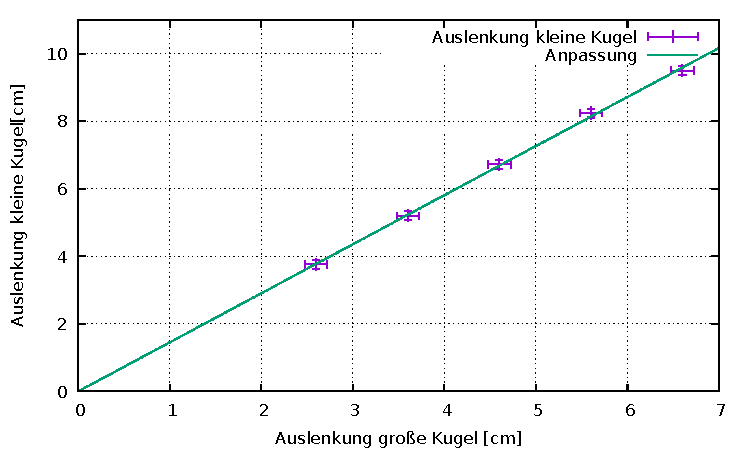
\includegraphics[width=0.8\textwidth]{res/GrosKlein.pdf}
	\caption{Zu sehen ist die Auslenkung der kleinen Kugel in Abhängigkeit von der Auslenkung der großen Kugel.}
	\label{fig:grosklein}
\end{figure}
\begin{figure}[h]
	\centering
	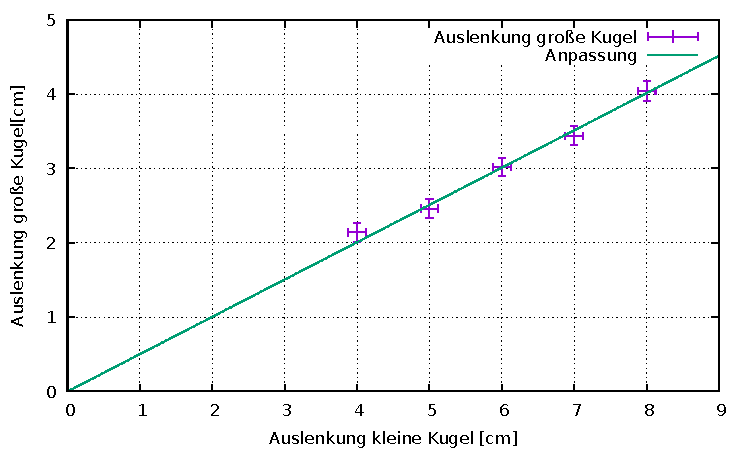
\includegraphics[width=0.8\textwidth]{res/KleinGros.pdf}
	\caption{Zu sehen ist die Auslenkung der großen Kugel in Abhängigkeit von der Auslenkung der kleinen Kugel.}
	\label{fig:kleingros}
\end{figure}

Die bei den fünf Messreihen erhaltenen Messwerte wurden jeweils gemittelt und sind in den Abbildungen \ref{fig:grosklein} und \ref{fig:kleingros} zu sehen. Die Fehlerbalken ergeben sich aus den Gleichungen \ref{eq:sud}, \ref{eq:sunv} und \ref{eq:kombsu} wobei von einer Messungenauigkeit von \SI{+-3}{mm} ausgegangen wurde.
Man erkennt das die Messwerte linear ansteigen. Da dies mit der Theorie übereinstimmt (Die Auslenkung nach dem Stoß ist durch
\begin{align}
	a_2= \frac{2m_1}{m_1+m_2} a_1\label{eq:Auslenkung}
\end{align} 
gegeben wobei $m_1$ die Masse der ausgelenkten Kugel ist und $a_1$ die Auslenkung von $m_1$.)
wurden die Messwerte mit der Linearen Anpassung\footnotetext{Die Anpassung wurde durch „Gnuplot“ mit dem Levenberg–Marquardt Algorithmus vorgenommen.} $a_2=b*a_1$ angepasst und die Unsicherheit der Anpassung wurde aus Gnuplot übernommen.
Um die Ergebnisse zu überprüfen wurde die Steigung $b$ aus den Massen der Kugeln bestimmt. Die Unsicherheit der Masse, ist durch die Anzeigeungenauigkeit der Digitalen Waage, die auf zwei Nachkommastellen genau anzeigt, gegeben. Und somit folgt mit den Gleichungen \ref{eq:sur} und \ref{eq:kombsu} die für die den Massen berechnete Steigung Unsicherheit. Der Vergleich der Werte ist in Tabelle \ref{tab:steigung} zu sehen.
Man erkennt, dass die Werte zwar voneinander Abweichen jedoch nur um ca. $3\%$ (Groß gegen Klein) bzw. um ca. $2\%$ (Klein gegen Groß). Dies ist darauf zurückzuführen, dass es sich bei dem untersuchten Stoß nicht um einen perfekten elastischen Stoß handelte bzw. das die Pendel nicht immer tatsächlich vollkommen ruhig hingen.
Über das Verhältnis der Steigungen der Anpassungsfunktion erhält man ein auch das Gewichtsverhältnis, dass sich über: 
\begin{align}
\frac{b_1}{b_2}=\frac{m_1}{m_2}	
\end{align} 
($b_1$, $m_1$ Steigung bzw. ausgelenktes Gewicht aus Abb. \ref{fig:grosklein} und $b_2$,$m_3$ Steigung bzw ausgelenktes Gewicht aus Abb. \ref{fig:kleingros} ) berechnen lässt. die Ergebnisse sind in Tabelle \ref{tab:Gewicht} zu sehen.
Man sieht ,dass das aus den Massen berechnete Gewichtsverhältnis  noch innerhalb der Unsicherheit des aus den Steigungen berechneten Verhältnisses liegt. Dies lässt darauf schließen, dass dieses Verfahren recht genau ist.

\begin{table}[h]
	\caption{Zu sehen sind die Steigungen der in Abb. \ref{fig:grosklein} und \ref{fig:kleingros} zu sehenden Anpassungsgeraden.}
	\begin{tabular}{|c|c|c|}
		\hline
		& Steigung Theoretisch & Steigung Experimentell\\
		& bestimmt & bestimmt\\
		\hline
		Groß gegen Klein &  \SI{1,487+-0,0002}{} & \SI{1,453+-0,016}{} \\
		\hline
		Klein gegen Groß & $0,513 \pm 6 \cdot 10^{-5}$&\SI{0,502+-0,006}{}\\
		\hline
	\end{tabular}
\label{tab:steigung}
\end{table}

\begin{table}[h]
	\caption{Zu sehen ist hier das Gewichtsverhältnis der Kleinen Kugel zur Großen Kugel.}
	\begin{tabular}{|c|c|}
		\hline
		Gewichtsverhätnis aus  & Gewichtsverhältnis aus\\
		 den Gewichten & der Steigung\\
		\hline
		$0,3451 \pm 6 \cdot 10^{-6}$& \SI{0,3455+-0,004}{}\\
		\hline
	\end{tabular}
	\label{tab:Gewicht}
\end{table}
